\documentclass[10pt,]{article}
\usepackage{lmodern}
\usepackage{setspace}
\setstretch{1.5}
\usepackage{amssymb,amsmath}
\usepackage{ifxetex,ifluatex}
\usepackage{fixltx2e} % provides \textsubscript
\ifnum 0\ifxetex 1\fi\ifluatex 1\fi=0 % if pdftex
  \usepackage[T1]{fontenc}
  \usepackage[utf8]{inputenc}
\else % if luatex or xelatex
  \ifxetex
    \usepackage{mathspec}
  \else
    \usepackage{fontspec}
  \fi
  \defaultfontfeatures{Ligatures=TeX,Scale=MatchLowercase}
\fi
% use upquote if available, for straight quotes in verbatim environments
\IfFileExists{upquote.sty}{\usepackage{upquote}}{}
% use microtype if available
\IfFileExists{microtype.sty}{%
\usepackage{microtype}
\UseMicrotypeSet[protrusion]{basicmath} % disable protrusion for tt fonts
}{}
\usepackage[margin=1in]{geometry}
\usepackage{hyperref}
\hypersetup{unicode=true,
            pdfborder={0 0 0},
            breaklinks=true}
\urlstyle{same}  % don't use monospace font for urls
\usepackage{longtable,booktabs}
\usepackage{graphicx,grffile}
\makeatletter
\def\maxwidth{\ifdim\Gin@nat@width>\linewidth\linewidth\else\Gin@nat@width\fi}
\def\maxheight{\ifdim\Gin@nat@height>\textheight\textheight\else\Gin@nat@height\fi}
\makeatother
% Scale images if necessary, so that they will not overflow the page
% margins by default, and it is still possible to overwrite the defaults
% using explicit options in \includegraphics[width, height, ...]{}
\setkeys{Gin}{width=\maxwidth,height=\maxheight,keepaspectratio}
\IfFileExists{parskip.sty}{%
\usepackage{parskip}
}{% else
\setlength{\parindent}{0pt}
\setlength{\parskip}{6pt plus 2pt minus 1pt}
}
\setlength{\emergencystretch}{3em}  % prevent overfull lines
\providecommand{\tightlist}{%
  \setlength{\itemsep}{0pt}\setlength{\parskip}{0pt}}
\setcounter{secnumdepth}{0}
% Redefines (sub)paragraphs to behave more like sections
\ifx\paragraph\undefined\else
\let\oldparagraph\paragraph
\renewcommand{\paragraph}[1]{\oldparagraph{#1}\mbox{}}
\fi
\ifx\subparagraph\undefined\else
\let\oldsubparagraph\subparagraph
\renewcommand{\subparagraph}[1]{\oldsubparagraph{#1}\mbox{}}
\fi

%%% Use protect on footnotes to avoid problems with footnotes in titles
\let\rmarkdownfootnote\footnote%
\def\footnote{\protect\rmarkdownfootnote}

%%% Change title format to be more compact
\usepackage{titling}

% Create subtitle command for use in maketitle
\providecommand{\subtitle}[1]{
  \posttitle{
    \begin{center}\large#1\end{center}
    }
}

\setlength{\droptitle}{-2em}

  \title{}
    \pretitle{\vspace{\droptitle}}
  \posttitle{}
    \author{}
    \preauthor{}\postauthor{}
    \date{}
    \predate{}\postdate{}
  
\usepackage{geometry}
\geometry{verbose,letterpaper,top=0.85in,left=2.75in,footskip=0.75in,marginparwidth=2in}

% \usepackage[breaklinks=true,pdfstartview=FitH,citecolor=blue]{hyperref}
\hypersetup{colorlinks,%
	citecolor=blue,%
	filecolor=red,%
	linkcolor=blue,%
	urlcolor=red,%
	pdfstartview=FitH}

\usepackage[T1]{fontenc}
\usepackage[utf8]{inputenc}
\usepackage{textgreek}
\usepackage[greek,english]{babel}
\usepackage{microtype}
\usepackage{amsmath}
\usepackage[osf]{libertine}
\usepackage{libertinust1math}
\usepackage{inconsolata}

\usepackage{booktabs}

\usepackage{setspace}
\doublespacing

% \setstretch{1.8999999999999999}

\usepackage[right]{lineno}

% \renewcommand{\rmdefault}{cmr}

% Additional template based on: https://www.overleaf.com/project/5dba26749d2ef50001d3a002

% clean citations
\usepackage{cite}

% hyperref makes references clicky. use \url{www.example.com} or \href{www.example.com}{description} to add a clicky url
\usepackage{nameref,hyperref}

% improves typesetting in LaTeX
\usepackage{microtype}
\DisableLigatures[f]{encoding = *, family = * }

% text layout - change as needed
\raggedright
\setlength{\parindent}{0.5cm}
\textwidth 5.25in 
\textheight 8.75in

% adjust caption style
\usepackage[aboveskip=1pt,labelfont=bf,labelsep=period,singlelinecheck=off]{caption}

% remove brackets from references
\makeatletter
\renewcommand{\@biblabel}[1]{\quad#1.}
\makeatother

% headrule, footrule and page numbers
\usepackage{lastpage,fancyhdr,graphicx}
\usepackage{epstopdf}
\pagestyle{myheadings}
\pagestyle{fancy}
\fancyhf{}
\rfoot{\thepage/\pageref{LastPage}}
\renewcommand{\footrule}{\hrule height 2pt \vspace{2mm}}
\fancyheadoffset[L]{2.25in}
\fancyfootoffset[L]{2.25in}

% use \textcolor{color}{text} for colored text (e.g. highlight to-do areas)
\usepackage{color}

% define custom colors (this one is for figure captions)
\definecolor{Gray}{gray}{.25}

% this is required to include graphics
\usepackage{graphicx}

% use if you want to put caption to the side of the figure - see example in text
\usepackage{sidecap}

% use for have text wrap around figures
\usepackage{wrapfig}
\usepackage[pscoord]{eso-pic}
\usepackage[fulladjust]{marginnote}
\reversemarginpar


% flush left while keep identation
\makeatletter
\newcommand\iraggedright{%
  \let\\\@centercr\@rightskip\@flushglue \rightskip\@rightskip
  \leftskip\z@skip}
\makeatother

% make pdf as default figure format
\DeclareGraphicsExtensions{.pdf,.png, %
    .jpg,.mps,.jpeg,.jbig2,.jb2,.JPG,.JPEG,.JBIG2,.JB2}

\begin{document}

% align only at left, not at right.
\iraggedright

\begin{flushleft}
{\Large
\textbf\newline{World record progression in track}
}
\newline
\\
Christopher D. Muir\textsuperscript{1,*},
Author 2\textsuperscript{2},
Author 3\textsuperscript{1},
Author 4\textsuperscript{1},
Author 5\textsuperscript{2},
Author 6\textsuperscript{2},
Author 7\textsuperscript{1}
\\
\bigskip
\bf{1} School of Life Sciences, University of Hawai\`{}i at M\=anoa, Honolulu, HI, USA
\\
\bf{2} Affiliation B
\\
\bigskip
* cdmuir@hawaii.edu

\end{flushleft}

\hypertarget{abstract}{%
\section{Abstract}\label{abstract}}

\begin{enumerate}
\def\labelenumi{\arabic{enumi}.}
\tightlist
\item
  the research conducted, including the rationale
\item
  methods
\item
  key results
\item
  the main conclusion, including the key points of discussion
\end{enumerate}

\linenumbers

\hypertarget{introduction}{%
\section{Introduction}\label{introduction}}

How fast can people run compared to other animals (Denny \protect\hyperlink{ref-denny_limits_2008}{2008})?

\hypertarget{methods}{%
\section{Methods}\label{methods}}

\hypertarget{subsection-1}{%
\subsection{Subsection 1}\label{subsection-1}}

I looked at how athletic world records changed through time.

\hypertarget{subsection-2}{%
\subsection{Subsection 2}\label{subsection-2}}

The second \protect\hyperlink{methods}{Methods} subsection.

\hypertarget{results}{%
\section{Results}\label{results}}

\marginpar{
\vspace{.7cm} % adjust vertical position relative to text with \vspace{} - note that you can enter negative numbers to move margin caption up
\color{Gray} % this gives caption a grey color to set it apart from text body
\textbf{Figure \ref{m100_1}. Example of a margin caption.} % note that \ref{fig1} refers to the corresponding wrapfigure
Setting up your figure + caption like this looks fancy and does not disrupt the flow of the text. But it requires more manual adjustments (position, spacing, labeling) compared to using standard \LaTeX figure environments.
}
\begin{wrapfigure}[12]{l}{75mm}
% the number in [] of wrapfigure is optional and gives the number of text lines that should be wrapped around the text. Adjust according to your figures height
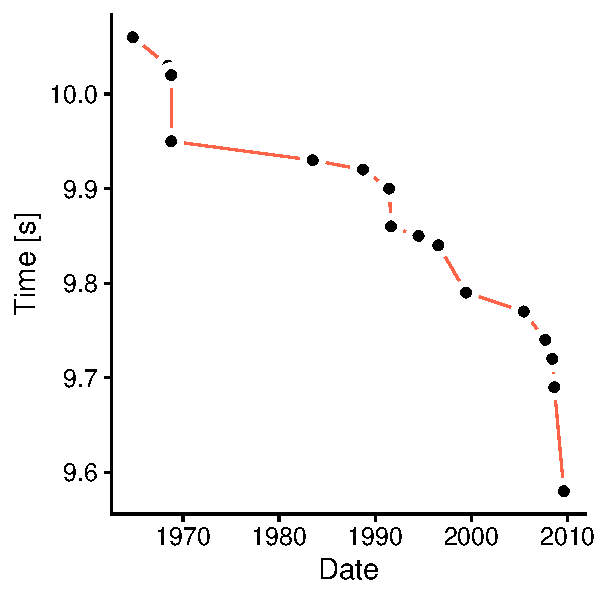
\includegraphics[width=75mm]{../figures/m100-progression.pdf}
\captionsetup{labelformat=empty} % makes sure dummy caption is blank
% add dummy caption - otherwise \label won't work and figure numbering will not count up
 \caption{}
\label{m100_1}
\end{wrapfigure}

Lorem ipsum dolor sit amet, consectetur adipiscing elit. Aliquam bibendum finibus diam, gravida sagittis lorem gravida vitae. Interdum et malesuada fames ac ante ipsum primis in faucibus. Nulla in diam tristique ante posuere tristique. Donec interdum purus sit amet nisl accumsan consectetur. Fusce aliquet libero mi, quis ornare dolor congue ullamcorper. Nulla nulla urna, molestie in urna sed, lacinia volutpat eros. Ut mi libero, elementum scelerisque ipsum vel, hendrerit fermentum turpis. Aliquam sit amet leo sodales, egestas augue id, fermentum nulla. Aenean vel cursus ante, et pellentesque eros. Nulla ac neque nec justo posuere commodo sit amet sit amet justo. Aliquam tincidunt tempor ex nec tincidunt. In ullamcorper vehicula lobortis.

\hypertarget{subsection-1-1}{%
\subsection{Subsection 1}\label{subsection-1-1}}

The first \protect\hyperlink{results}{Results} subsection.

\hypertarget{subsection-2-1}{%
\subsection{Subsection 2}\label{subsection-2-1}}

The second \protect\hyperlink{results}{Results} subsection. See Figure \ref{m100_2}

Lorem ipsum dolor sit amet, consectetur adipiscing elit. Aliquam bibendum finibus diam, gravida sagittis lorem gravida vitae. Interdum et malesuada fames ac ante ipsum primis in faucibus. Nulla in diam tristique ante posuere tristique. Donec interdum purus sit amet nisl accumsan consectetur. Fusce aliquet libero mi, quis ornare dolor congue ullamcorper. Nulla nulla urna, molestie in urna sed, lacinia volutpat eros. Ut mi libero, elementum scelerisque ipsum vel, hendrerit fermentum turpis. Aliquam sit amet leo sodales, egestas augue id, fermentum nulla. Aenean vel cursus ante, et pellentesque eros. Nulla ac neque nec justo posuere commodo sit amet sit amet justo. Aliquam tincidunt tempor ex nec tincidunt. In ullamcorper vehicula lobortis.

\begin{figure}[ht]
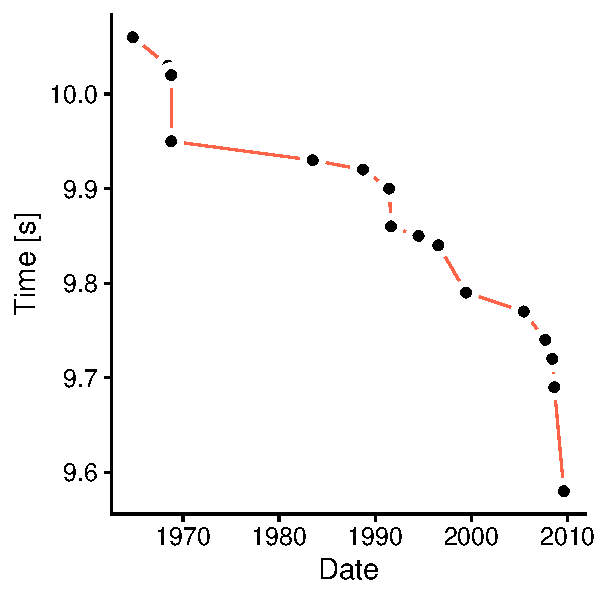
\includegraphics[width=\textwidth]{../figures/m100-progression.pdf}
\caption{\color{Gray} \textbf{Example of a standard floating figure}. \textbf{A-F}, This figure is wrapped into the standard floating environment.}
\label{m100_2}
\end{figure}

\hypertarget{discussion}{%
\section{Discussion}\label{discussion}}

People are getting faster!

\hypertarget{references}{%
\section*{References}\label{references}}
\addcontentsline{toc}{section}{References}

\hypertarget{refs}{}
\leavevmode\hypertarget{ref-denny_limits_2008}{}%
Denny, Mark W. 2008. ``Limits to Running Speed in Dogs, Horses and Humans.'' \emph{The Journal of Experimental Biology} 211 (24): 3836--49.


\end{document}
